\documentclass[DIN, pagenumber=false, fontsize=11pt, parskip=half]{scrartcl}

\usepackage{amsmath}
\usepackage{amsfonts}
\usepackage{amssymb}
\usepackage{enumitem}
\usepackage[utf8]{inputenc} 
\usepackage[ngerman]{babel} 
\usepackage[T1]{fontenc} 
\usepackage{pgfplots}
\usepackage{xcolor}
\usepackage{listings}
\usepackage{float}
\usepackage{graphicx}
\usepackage{booktabs}

\definecolor{mygreen}{RGB}{28,172,0} % color values Red, Green, Blue
\definecolor{mylilas}{RGB}{170,55,241}

\tikzstyle{neuron}=[circle,fill=black!25,minimum size=30pt,inner sep=0pt]

\lstset{language=Matlab,%
    %basicstyle=\color{red},
    breaklines=true,%
    morekeywords={matlab2tikz},
    keywordstyle=\color{blue},%
    morekeywords=[2]{1}, keywordstyle=[2]{\color{black}},
    identifierstyle=\color{black},%
    stringstyle=\color{mylilas},
    commentstyle=\color{mygreen},%
    showstringspaces=false,%without this there will be a symbol in the places where there is a space
    numbers=left,%
    numberstyle={\tiny \color{black}},% size of the numbers
    numbersep=9pt, % this defines how far the numbers are from the text
    emph=[1]{for,end,break},emphstyle=[1]\color{red}, %some words to emphasise
    %emph=[2]{word1,word2}, emphstyle=[2]{style},    
}

\title{Einführung in die Neuroinformatik}
\author{Tim Luchterhand, Paul Nykiel (Gruppe P)}

\begin{document}
    \maketitle
    \section{Lernregeln}
    \subsection{}
    \begin{eqnarray*}
        && \frac{\partial E}{\partial w} = \frac{\partial}{\partial w}\left( \frac{1}{2} \sum_{\mu=1}^M {(T^\mu - f(w \cdot x^\mu +b))}^2 \right) \\
        &=& \sum_{\mu=1}^M \frac{1}{2} \cdot 2 (T^\mu - f(w \cdot x^\mu + b)) \cdot (-f'(w \cdot x^\mu + b)) \cdot x^\mu \\
        &=& - \sum_{\mu=1}^M (T^\mu - f(w \cdot x^\mu + b)) \cdot f'(w \cdot x^\mu + b) \cdot x^\mu
    \end{eqnarray*}
    \begin{eqnarray*}
        && \frac{\partial E}{\partial b} = \frac{\partial}{\partial b}\left( \frac{1}{2} \sum_{\mu=1}^M {(T^\mu - f(w \cdot x^\mu +b))}^2 \right) \\
        &=& \sum_{\mu=1}^M \frac{1}{2} \cdot 2 (T^\mu - f(w \cdot x^\mu + b)) \cdot (-f'(w \cdot x^\mu + b))\\
        &=& - \sum_{\mu=1}^M (T^\mu - f(w \cdot x^\mu + b)) \cdot f'(w \cdot x^\mu + b)
    \end{eqnarray*}
    \subsection{}
    \begin{enumerate}[label=(\alph*)]
        \item Inkrementelle Version:
            \begin{eqnarray*}
                w(t+1) &=& w(t) + \eta \cdot (T^\mu - f(w \cdot x^\mu + b)) \cdot f'(w \cdot x^\mu + b) \cdot x^\mu \\
                b(t+1) &=& b(t) + \eta \cdot  (T^\mu - f(w \cdot x^\mu + b)) \cdot f'(w \cdot x^\mu + b) 
            \end{eqnarray*}
        \item Batch Version:
            \begin{eqnarray*}
                w(t+1) &=& w(t) + \eta \cdot \sum_{\mu=1}^M (T^\mu - f(w \cdot x^\mu + b)) \cdot f'(w \cdot x^\mu + b) \cdot x^\mu \\
                b(t+1) &=& b(t) + \eta \cdot \sum_{\mu=1}^M (T^\mu - f(w \cdot x^\mu + b)) \cdot f'(w \cdot x^\mu + b) 
            \end{eqnarray*}
    \end{enumerate}
    \subsection{}
    \begin{enumerate}[label=(\alph*)]
        \item
            Ableitung der Transferfunktion:
            \begin{equation*}
                f'(x) = -\frac{e^{-x}}{{(1+e^{-x})}^2}
            \end{equation*}
            % Berechnen mit JS:
            % var f = x => 1/(1+Math.exp(-x))
            % var f_ = x => -Math.exp(-x)/Math.pow(1+Math.exp(-x),2)
            % f(2)*f_(2)+2*f(1)*f_(1)-f(4)*f_(4)
            % f(4)*f_(4)+f(2)*f_(2)*+f(1)*f_(1)

            Werte des Gradienten berechenen:
            \begin{eqnarray*}
                \frac{\partial E}{\partial w}(-1,3) &=& - \sum_{\mu=1}^4 (T^\mu - f(-1 \cdot x^\mu + 3)) \cdot f'(-1 \cdot x^\mu + 3) \cdot x^\mu\\ 
                &=& - \left(((0-f(4)) \cdot f'(4) \cdot -1) + 0 + ((0-f(2)) \cdot f'(2) \cdot 1) + ((0-f(1)) \cdot f'(1) \cdot 2)\right) \\
                &=& - \left(f(4)f'(4) -f(2)f'(2)-2f(1)f'(1) \right) \\
                &=&  f(2)f'(2) + 2f(1)f'(1) -f(4)f'(4)\\
                &=& -0.36 \\
                \frac{\partial E}{\partial b}(-1,3) &=& - \sum_{\mu=1}^4 (T^\mu - f(-1 \cdot x^\mu + 3)) \cdot f'(-1 \cdot x^\mu + 3) \\
                &=& - \left(((0-f(4)) \cdot f'(4)) + 0 + ((0-f(2)) \cdot f'(2)) + ((0-f(1)) \cdot f'(1))\right) \\
                &=& f(4)f'(4) + f(2)f'(2) + f(1)f'(1) \\
                &=& -0.0041
            \end{eqnarray*}
            \begin{equation*}
                \Rightarrow \nabla E(w(0),b(0)) = \begin{pmatrix}
                    -0.36 \\ -0.0041
                \end{pmatrix}
            \end{equation*}
        \item $ $
            \begin{figure}[H]
                \centering
                \begin{tikzpicture}
                    \node at (0,0) {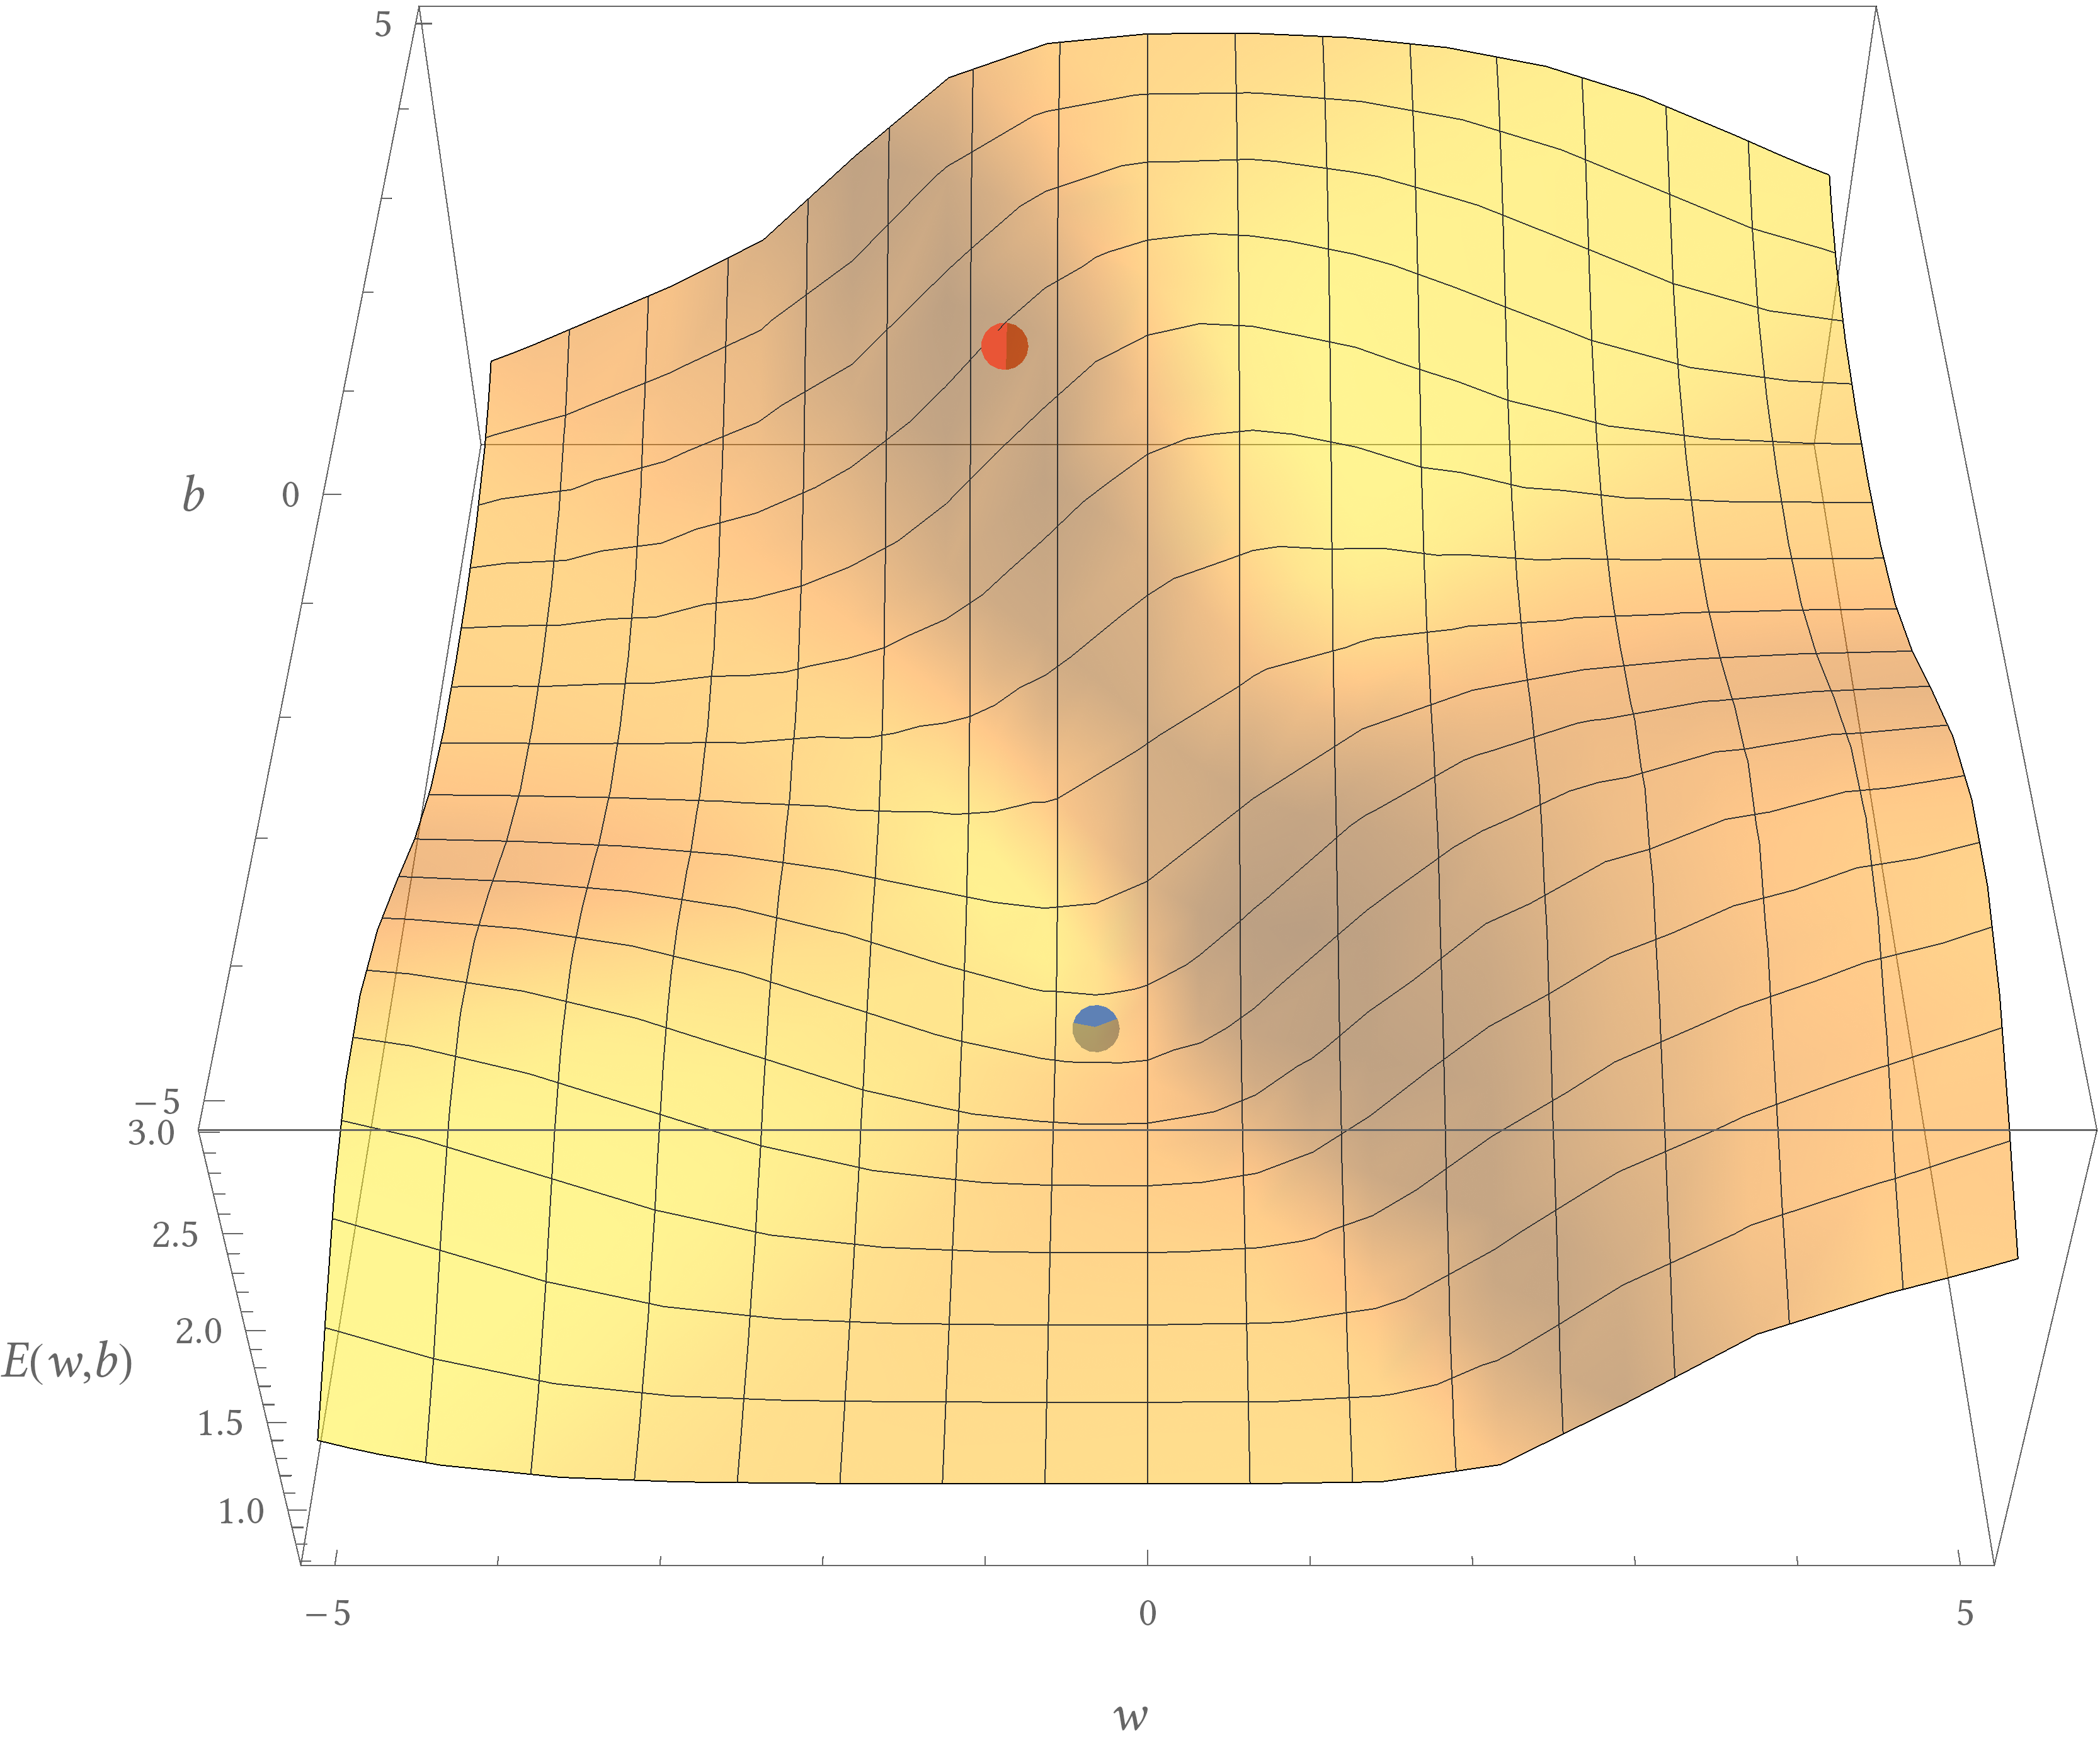
\includegraphics[width=\textwidth]{gradient.png}};
                    \draw[thick, ->, color=black] (-0.3,3.7) -- (-1.0,3);
                \end{tikzpicture}
                \caption{Richtung des Gradienten}
            \end{figure}
        \item
            \begin{eqnarray*}
                w(1) &=& w(0) - \eta \cdot \frac{\partial E}{\partial w}(w(0),b(0)) \\
                &=& -1 - 0.8 \cdot (-0.36) \\
                &=& -0.712 \\
                b(1) &=& b(0) - \eta \cdot \frac{\partial E}{\partial b}(w(0), b(0)) \\
                &=& 3 - 0.8 \cdot (-0.0041) \\
                &=& 3.0033
            \end{eqnarray*}
        \item Der Gradientenabstieg findet nicht das globale Minimum sondern nur ein lokales Minimum, denn dort ist der Gradient aber ebenfalls $\vec{0}$.
    \end{enumerate}
    \subsection{}
    \begin{enumerate}[label=(\alph*)]
        \item Pfad 1 ist vermutlich durch die Batch-Lernregel entstanden, Pfad 2 durch die inkrementelle Lernregel. 

            Da bei der Batch-Lernregel der Gradient aus vielen Trainingssamples berechnet wird (also eine Art Durchscnitt), springt der Pfad weniger.
            Bei der inkrementellen Lernregel hingegen beeinflussen die einzelnen Trainingspaare den Pfad jeweils maßgeblich. Bei jeder Iteration wird nur genau ein Sample berücksichtigt, alle anderen Samples haben keinen Einfluss. Dadurch ist der Pfad deutlich weniger glatt, als bei der Batch-Lernregel.

        \item Es ist möglich, dass beim inkrementellen Lernen kein globales Minimum gefunden wird, obwohl das Batch-Lernverfahren erfolgreich war. In dem Fall könnte das inkrementelle Lernen nur ein Minimum, welches für eine bestimmte Teilmenge der Traininssamples gut passt, gefunden haben. Andererseits könnte das Batch-Lernverfahren nur ein lokales Minnimu finden währen das inkrementelle Lernverfahren \glqq{}zufällig\grqq{} über dieses hinausspringt und noch weiter absteigen kann.
    \end{enumerate}
    \subsection{}
    Bei zu großer Lernrate kann die Minimierung der Fehlerfunktion zu einer Art überschwingen oder sogar zu einer Oszillation führen. Da der Pfad immer zu weit \glqq{}springt\grqq{} erreicht er somit nie das Minimum.
    \subsection{}
    Es wird versucht die Übertragungsfunktion des Neurons so anzupassen, dass sie möglichst nah an allen Punkten ist. Die Funktion hat jedoch immer eine Sigmoid-Form und lässt sich durch das Training nur verschieben sowie strecken/stauchen. Da die Funktion aber streng monoton ist, kann sie so nie alle Punkte optimal annähern.
\end{document}
